
\documentclass[
	article,			% indica que é um artigo acadêmico
	11pt,				% tamanho da fonte
	oneside,			% para impressão apenas no verso. Oposto a twoside
	a4paper,			% tamanho do papel. 
	english,			% idioma adicional para hifenização
	brazil,				% o último idioma é o principal do documento
	]{abntex2}


\usepackage{cmap}				% Mapear caracteres especiais no PDF
\usepackage{lmodern}			% Usa a fonte Latin Modern
\usepackage[T1]{fontenc}		% Seleção de códigos de fonte.
\usepackage[utf8]{inputenc}		% Codificação do documento (conversão automática dos acentos)
\usepackage{indentfirst}		% Indenta o primeiro parágrafo de cada seção.
\usepackage{nomencl} 			% Lista de símbolos
\usepackage{color}				% Controle das cores
\usepackage{graphicx}			% Inclusão de gráficos

\usepackage{lipsum}				% para geração de dummy text
\usepackage{synttree}

\usepackage[brazilian,hyperpageref]{backref}	 % Paginas com as citações na bibl
\usepackage[alf]{abntex2cite}	% Citações padrão ABNT

\renewcommand{\backrefpagesname}{Citado na(s) página(s):~}

\renewcommand{\backref}{}
\renewcommand{\thesubsection}{\thesection.\alph{subsection}}

\renewcommand*{\backrefalt}[4]{
	\ifcase #1 %
		Nenhuma citação no texto.%
	\or
		Citado na página #2.%
	\else
		Citado #1 vezes nas páginas #2.%
	\fi}%

\titulo{Avaliação de Expressões}
\autor{Diego P. da Jornada\thanks{diego.jornada@acad.pucrs.br}\and Milton C. de Oliveira\thanks{milton.oliveira@acad.pucrs.br}}

\definecolor{blue}{RGB}{41,5,195}

\makeatletter
\hypersetup{
		pdftitle={\@title}, 
		pdfauthor={\@author},
    	pdfsubject={Modelo de artigo científico com abnTeX2},
	    pdfcreator={LaTeX with abnTeX2},
		pdfkeywords={abnt}{latex}{abntex}{abntex2}{atigo científico}, 
		colorlinks=true,       		% false: boxed links; true: colored links
    	linkcolor=blue,          	% color of internal links
    	citecolor=blue,        		% color of links to bibliography
    	filecolor=magenta,      		% color of file links
		urlcolor=blue,
		bookmarksdepth=4
}
\makeatother

\makeindex

\setlrmarginsandblock{4cm}{4cm}{*}
\setulmarginsandblock{4cm}{4cm}{*}
\checkandfixthelayout

\setlength{\parindent}{1.3cm}

\setlength{\parskip}{0.2cm}  % tente também \onelineskip

\SingleSpacing

\begin{document}

\frenchspacing 

\maketitle

\begin{resumoumacoluna}
    
    Este artigo descreve as soluções para a segunda tarefa realizada na disciplina de \emph{Paradigmas de Linguagens de Programação} de 2015/1

 \vspace{\onelineskip}
 
 \noindent
\end{resumoumacoluna}

\textual

    \section*{Introdução}

        Dentro do escopo da disciplina de \emph{Paradigmas de Linguagens de Programação} o segundo trabalho é o seguinte: solucionar os exercícios sobre avaliação de expressões que foram propostos no escopo da tarefa.
        
    \section{Exercício Um}
    
        
        \subsection{}
        \begin{center}
        \synttree
            [
            <bloco>
                [\{]
                [<linha> [<instrucao> [<var> [C]] [.x :=] [<exp> [<exp1> [B]]] ] [;]]
                [<linha> [<instrucao> [<var> [A]] [.x :=] [<exp> [exp2 [<var> [C]] [<op> [*]][<const> [2]]]] [;]]]
                [\}]
            ]
        \end{center}
            
        \subsection{}
            \begin{center}
            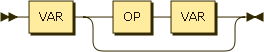
\includegraphics[scale=.75]{EXP1} 
            \end{center}
\pagebreak
    \section{Exercício Dois}
        \subsection{}
        \paragraph{Árvode de Derivação:}
            \begin{center}
            \synttree[/[*[3][x]] [-[* [4] [*[x][z]]] [\^ [y] [3]]]]
            \end{center}
            
        \paragraph{Notação de Prefixo:} / * 3 x - * 4 * x 2 \^\ y 3
        \paragraph{Notação de Sufixo:} 3 x * 4 x z * * y 3 \^\ - /
        
        \subsection{}
        \paragraph{Árvode de Derivação:}
            \begin{center}
            \synttree[/ [+ [/ [+ [2] [x]] [y]] [2]] [x]]
            \end{center}
            
        \paragraph{Notação de Prefixo:} / + / + 2 x y 2 x
        \paragraph{Notação de Sufixo:} 2 x + y / 2 + x /
\pagebreak
        \subsection{}
        \paragraph{Árvode de Derivação:}
            \begin{center}
            \synttree[- [\^ [\^ [\^ [x] [3]] [3]] [3]] [2]]
            \end{center}
            
        \paragraph{Notação de Prefixo:} - \^\ \^\ \^\ x 3 3 3 2 
        \paragraph{Notação de Sufixo:} x 3 \^\ 3 \^\ 3 \^\ 2 -
    \section{Exercício Três}
    
    x y - z + w /

\end{document}